\chapter{Fundamento te'orico}
\label{capitulodos}
Las p'aginas web han mejorado continuamente en la disponibilidad de la informaci'on a tr'aves de los servicios web denominado SOA \footnote{SOA- Arquitectura orientado a servicios}, los cuales  utilizan el protocolo de comunicaci'on para que la aplicaci'on m'ovil pueda realizar una solicitud al servicio web.

\section{Sistemas Distribuidos}

Los sistemas distribuidos son un conjunto de computadoras independientes para mostrar a los usuarios como un solo sistema en diferentes dispositivos tanto en hardware como en software y se comunican en red para coordinar sus acciones mediante el envi'o de mensaje(Colourios, 2012).\cite{Colourios2012}

Seg'un Colourios las ventajas para utilizar un sistema distribuido son:
\begin{enumerate}
\item \textbf{El intercambio de recursos:} es aquella que permite compartir hardware y software de sus recursos a tr'aves de la red.

\item \textbf{Las aperturas distribuidas:} se utilizan los dise'nos est'andares de protocolos.

\item \textbf{La concurrencia:} son los  procesos que podr'ian operar al mismo tiempo en computadoras separadas sobre la red. Estos procesos podr'ian comunicarse con otros, durante su operaci'on normal.

\item \textbf{La escalabilidad:} es aumentar nuevos recursos al sistema.
\end{enumerate}

El sistema distribuido se organiza como un sistema de cliente y servidor.

\subsection{Computaci'on cliente servidor}
La computaci'on de cliente servidor se refiere al usuario que interact'ua con un programa y se ejecuta en la computadora local. Este usuario interact'ua con un programa que se ejecuta en otra  computadora remota, el c'ual proporciona servicios como acceso a p'aginas web \cite{Somerville2011}. Como se muestra en la figura \ref{fig:clienteServidor}. 
%se han realizado modificaciones
\begin{figure}[H]
\centering
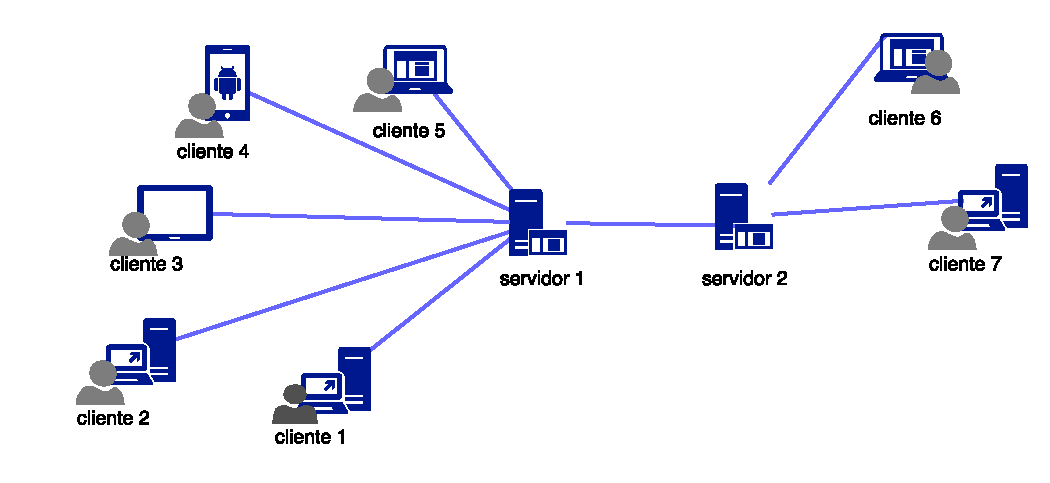
\includegraphics[width=0.6\textwidth]{clienteServidorP.pdf}
\captionsetup{justification=centering,margin=2cm}
\caption{Computaci'on cliente-servidor, adoptado para la realizac'ion del proyecto. Arquitectura cliente servidor de Somerville\cite{Somerville2011}}
\label{fig:clienteServidor}
\end{figure}

Para implementar un sistema cliente servidor tiene que instalar un programa en la computadora cliente para que se comunique con el servidor. Este cliente no tiene estado y no se implementa es como un conjunto de servicios independientes. Este cliente es conocido como SOA que se explica a continuaci'on.

\section{La arquitectura orientada a servicio web}
El arquitectura orientada a servicios es un componente de software de reutilizaci'on, debidamenta ajustado se accede de manera program'atica. \cite{Somerville2011}. Como se muestra en la figura \ref{fig:ArquitecturaSOA}.

\begin{figure}[H]
\centering
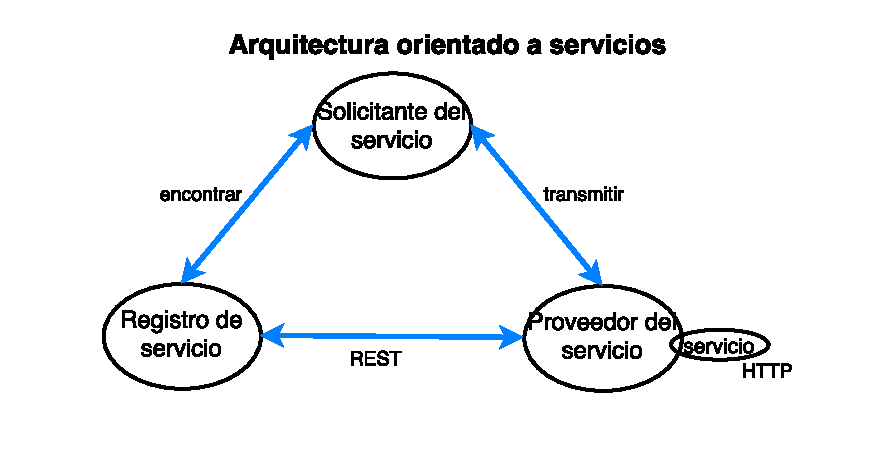
\includegraphics[width=0.4\textwidth]{arqSOA.pdf}
\captionsetup{justification=centering, margin=2cm}
\caption{Arquitectura orientado a servicio, adoptado para la realizac'ion del proyecto. El objetivo del SOA de Somerville \cite{Somerville2011}}
\label{fig:ArquitecturaSOA}
\end{figure}

Las caracter'isticas del servicio web son las siguientes:
\begin{enumerate}
\item Compartir informaci'on entre empresas.
\item La informaci'on debe tener una representaci'on est'andar.
\item Es indepediente de la aplicaci'on o sistema que usa el servicio web.
\item El servicio web es independiente de la plataforma y del lenguaje de implementaci'on.
\item Desde el principio, tiene un proceso est'andar para el servicio web en donde las compa'nias se han comprometido a dicho est'andar. 
\end{enumerate}

%Para el presente proyecto la implementaci'on y la interface del servicio, son definidos como un sistema heredado.

%\subsection{Sistema heredado}
%El sistema heredado es un sistema de software antiguo, donde es posible acceder a la funcionalidad del sistema mediante una nueva aplicaci'on que brinde acceso a las funciones y datos de un sistema heredado y utilizar nuevas tecnolog'ias\cite{Somerville2011}. Como se muestra en la figura \ref{fig:heredado}.

%\begin{figure}[H]
%\centering
%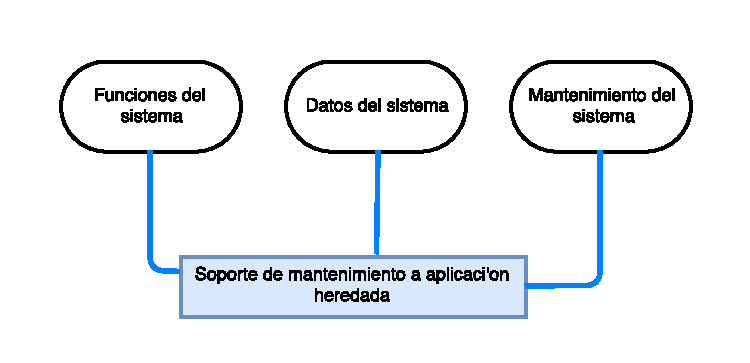
\includegraphics[width=0.5\textwidth]{servicioHeredado.pdf}
%\captionsetup{justification=centering, margin=2cm}
%\caption{Servicio heredado, adoptado para la realizac'ion del proyecto. Representaci'on de un servicio heredado de \cite{Somerville2011}}
%\label{fig:heredado}
%\end{figure}

La uni'on y la comunicaci'on entre el cliente y el servicio se realiza mediante diferentes  protocolos que se explicara continuaci'on.

\subsection{Protocolo de servicio}
El protocolo de servicio es un conjunto de reglas que se utilizan para la comunicaci'on e intercambio de informac'ion entre el protocolo mencionado anteriormente y a tr'aves de una red (Navarro, 2006).\cite{Navarro2006}. 
Seg'un Navarro los protocolos se dividen en dos tipos:
\begin{itemize}
\item Protocolos est'andares son : SOAP, WSDL \footnote{WSDL - Descripcion de lenguajes de servicios web}, WS-BPEL \footnote{WS-BPEL - Lenguaje de Ejecuci'on de procesos de negocio con servicios web}.
\item Protocolo no est'andar: el metodo REST.
\end{itemize}
 
Para el presente proyecto se ha utilizado el protocolo  REST se desarrolla en el siguiente parr'afo.

\section{Protocolo REST} 
El protocolo REST es un estilo de arquitectura de software que se refiere a una colecci'on de principios para el dise'no de arquitecturas en la red. El t'ermino frecuentemente es utilizado en el sentido de describir a cualquier interfaz que transmite datos espec'ificos de un dominio sobre HTTP\footnote{ HTTP- Hipertexto de Transferencia de Protocolo}. Se basa en est'andares de protocolo HTTP(Navarro, 2006).\cite{Navarro2006}.

\subsection{Protocolo HTTP}

El protoco HTTP es un conjunto de m'etodos de petici'on para indicar la acci'on que se desea realizar, en el recurso determinado cada uno de ellos implementan una sem'antica diferente, pero tienen alguna caracter'istica similar, las cuales son: Get, Head, Post, Put, Delete, Connect, Options, Trace y Patch.(Navarro, 2006) \cite{Navarro2006}. 

Seg'un Navarro, las funciones sobre la web que maneja HTTP son: el cache, los requisitos de origen,el proxie, el t'unel y sesi'on. \\

A continuaci'on se describen las funciones que se exploran en este proyecto.
\begin{enumerate}
\item \textbf{El cache:} es la funci'on para almacenar los documentos en la memoria del navegador. 
\item \textbf{ Requisitos de origen:} son funci'ones para compartir la informaci'on de datos y puede flexibilizar la informaci'on entre cliente y servidor. 
\item \textbf{La autentificaci'on:} es la funci'on que establece la sesi'on y almacena informaci'on en el cokie para guardar en el navegador. 
\end{enumerate}

\section{Unidad de datos del servicio}
La unidad de datos del servicio es un termino gen'erico para compartir informaci'on entre el servicio y el cliente. Estas unidades de datos pueden ser: Json\footnote{Json- Notaci'on de objetos de javascript}, Xml\footnote{XML-Lenguaje de Marcado Extensible} y Yaml \footnote{Yaml-Otro lenguaje de marcado m'as}. La unidad de datos Json se ha empleado en este proyecto se explica a continuaci'on.

\subsection{Json}
El Json es un formato ligero y abierto de intercambio de datos. Utiliza  el texto plano para compartir informaci'on, el c'ual es  independiente del lenguaje de programaci'on.  
Las estructura para compartir informaci'on pueden ser objetos o arreglo y tambi'en se puede combinar ambos, como se muestran en la figura \ref{fig:jsonO} y \ref{fig:jsonA} a continuaci'on.

\begin{figure}[H]
\begin{minipage}{0.48\textwidth}
\centering
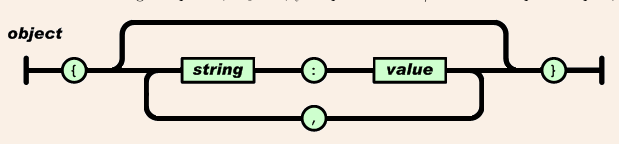
\includegraphics[width=0.8\textwidth]{jsonObj.png}
\captionsetup{justification=centering,margin=2cm}
\caption{Representaci'on de json por objeto, adoptado para la realizaci'on del proyecto. Estructura de json por objeto, de Figura: Elaboraci'on propia}
\label{fig:jsonO}
\end{minipage}\hfill
\begin {minipage}{0.48\textwidth}
\centering
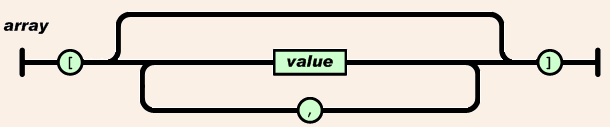
\includegraphics[width=0.8\textwidth]{jsonArr.png}
\captionsetup{justification=centering,margin=2cm}
\caption{Representaci'on del json por arreglo, adoptado para la realizaci'on del proyecto. Estructura de json por arreglo de Fuente: Elaboraci'on propia}
\label{fig:jsonA}
\end{minipage}
\end{figure}

\subsection{Json web token}
El json web token conocico como JWT\footnote{JWT - Json web token} es un m'etodo abierto y est'andar para representar las  solicitudes de forma segura entre dos partes. Este se dividen tres partes: la cabecera, la carga 'util y una firma.

\begin{figure}[H]
\centering
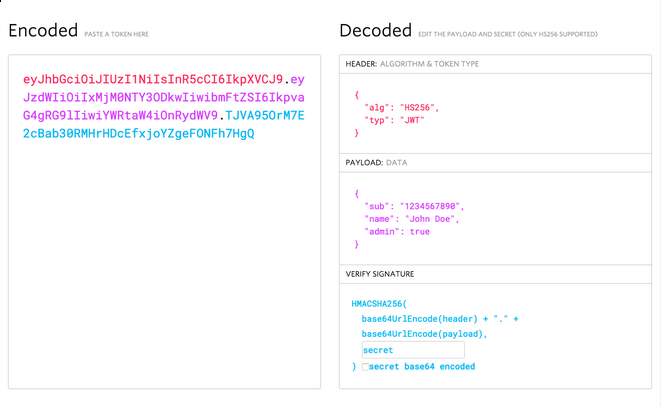
\includegraphics[width=0.6\textwidth]{arqJWT.png}
\captionsetup{justification=centering,margin=2cm}
\caption{ Representaci'on del json web token Fuente: Elaboraci'on propia}
\end{figure}

En este proyecto el tipo de servicio web es identificado como un servicio heredado porque realiza solicitud de datos para la aplicaci'on m'ovil.

\section{Las aplicaciones m'oviles}
Seg'un la corporaci'on de IBM \footnote{IBM - M'aquinas de negocios internacionale}  define a las aplicaciones m'oviles en tres partes, las cuales son: nativa, web y hibrido. \cite{Ibm2012}

\subsection{La aplicaci'on nativa}
La aplicaci'on nativa se conecta directamente con el sistema operativo m'ovil, sin ning'un intermediario ni contenedor. La aplicaci'on nativa puede acceder libremente a todas las Apis que el proveedor del sistema operativo ponga a su disposici'on y en muchos casos, tiene caracter'isticas y funciones 'unicas que son t'ipicas del sistema operativo m'ovil en particular.
%Nos hemos quedado aqui
\subsection{La aplicaci'on web}
La aplicacion web utiliza 'unicamente tecnolog'ias basadas en la web como ser la quinta version de HTML \footnote{HTML - Lenguaje de Marcado para Hipertexto}, el mismo tiene componente de interfaz de usuario avanzado, acceso a m'ultiples tipos de medios, servicios de geoposicionamiento y disponibilidad sin Internet.\\
Una ventaja de esta aplicaci'on es el soporte para m'ultiples plataformas y se ejecuta dentro del navegador.
\subsection{La aplicaci'on h'ibrida}
La aplicaci'on h'ibrida tiene un  enfoque h'ibrido que combina desarrollo nativo con tecnolog'ia web. La aplicaci'on hibrida utiliza  m'ultiples plataformas y tiene acceso a los dispositivos del celular tales son: la camara, acceso de dato, almacenamiento de informaci'on y otros.

En este proyecto se ha utilizado la aplicacion h'ibrida porque permite acceder a la parte nativa del m'ovil y almacena informaci'on en la aplicaci'on.

\section{Los dispositivos m'oviles}
Actualment'e, el dispositivo m'ovil es peque'no para ser manejado facilmente se ha utilizado durante su transporte. Se caracteriza por el mejoramiento que va adquiriendo su tama'no reducido, la telecomunicaci'on de software,  la gran iteracci'on entre las personas. Convirt'iendolos en una necesidad primaria para la sociedad\cite{Morillo2014}.\\
Desde su creaci'on  los dispositivos m'oviles han evolucionado en gran magnitud, es por eso que muchas empresas han ofrecido diferentes sistemas operativos como ser: android, ioS, Windows, etc. El sistema operativo de android se utiliza para el presente proyecto.

\subsection{El sistema operativo android}
E sistema operativo android basada en la  plataforma de software Linux para dispositivos m'oviles. 
El sistema operativo android es un sistema operativo libre y tiene acceso a sus recursos como la pantalla, camara y otros\cite{Android}. A continuaci'on consta con las siguientes capas, se muestra en la siguiente figura \ref{fig:Android}.

\begin{figure}[H]
\centering
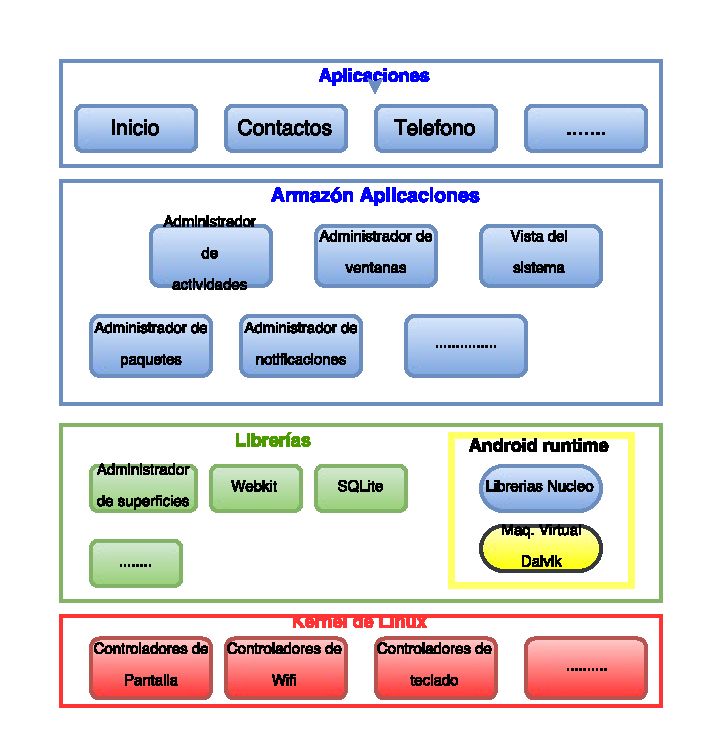
\includegraphics[width=0.3\textwidth]{capaAndroid.pdf}
\captionsetup{justification=centering, margin=2cm}
\caption{Capas del sistema operativo de android, adoptado para la realizac'ion del proyecto. Fuente: Introducci'on a Android  \cite{Android}}
\label{fig:Android}
\end{figure}

Con el avance de la tecnolog'ia han aumentado el incremento, en diferentes dispositivos como ser tablet PC, tablet, smartphone y otros el c'ual utilizan el sistema operativo android. 
%Debido a la diversidad de dispositivos m'oviles, para el presente proyecto se utiliza el dise'no adaptativo que se explica a continuaci'on.

%\section{El dise'no adaptativo}
%El dise'no adaptativo se refiere a la satisfacci'on de visitar una p'agina web a tr'aves de diferentes dispositivos, ha  generado la filosof'ia de  Responsive Web Design, este pensamiento fue establecida por Steven Champeon (2003), qui'en propone realizar un 'unico dise'no web para todos los dispositivos y accesible para todos los usuarios \cite{Adrian2012}.

\section{Las herramientas para las plataformas de desarrollo}
Las herramientas  para el desarrollo las cuales son: 'el entorno de desarrollo vim y 'el navegador de chrome.

\subsection{El entorno de desarrollo VIM}
Seg'un la p'agina oficial de Vim, el Vim se define como un editor de texto altamente configurable construido para creaciones y cambios de cualquier tipo de texto. Tiene las siguientes ventajas: persistente multinivel, extensivos plugin para el sistema, soportan diferentes lenguajes de programaci'on y diferentes formatos de archivos y otros.
\subsection{El navegador web - Chrome}
Es un navegador web r'apido, seguro y gratuito, dise'nado para la web actual, as'i lo define la p'agina oficial del mismo.
 
Tambi'en es un navegador para dispositivos m'oviles.  La ventaja que brinda es verificar los errores para celulares, minimizar los gastos de datos, almacenar la sesi'on y permitir crear base datos en el navegador.

\section{Herramientas de desarrollo}
Se utilizo tres framework los cuales son ionic, angularjs y nodejs. Estos se basan en el lenguaje de javaScript para la implementaci'on del servicio web y la aplicaci'on  m'ovil las cuales son:

\subsection{Framework ionic}
Seg'un la p'agina oficial de  ionic este framework es un SDK para HTML5 que nos ayuda a construir una aplicaci'on m'ovil h'ibrida usando las tecnolog'ias como HTML, CSS y Javascript. Se caracteriza por ser multiplataforma y utiliza el framework de angularJS.

\subsection{Framework angularJS}
Seg'un la p'agina oficial de angularJS este es un conjunto de  herramientas  para construir el framework  mas adecuado para desarrollo de aplicaciones. Es totalmente extensible y trabaja con otras librer'ias, cada caracter'istica puede ser modificado o remplazado, para adaptarse a su  flujo de trabajo.

\subsection{Framework node.js}
El framework de nodeJS es un entorno de ejecuci'on para javaScript construido con el motor JavaScript V8 de Chrome. Nodejs utiliza un modelo de operaci'on de E/S sin bloqueo y orientado a eventos que lo hace liviano y eficiente. El ecosistema de paquetes de Node.js, npm, es el ecosistema mas grande de librer'ias de c'odigo abierto en el mundo. Seg'un la p'agina oficial de nodejs.
%aumentado
Para el desarrollo de la aplicaci'on m'ovil se ha utilizado el framework ionic.
Ionic es de c'odigo libre y se basa en librer'ias orientadas 'unicamente a aplicaciones de dispositivos m'oviles. Tambi'en se enfocan a desarrollo de aplicaciones h'ibridas construida con HTML3, CSS3 y Javascript se construye p'aginas web, se ejecutan dentro de un navegador, el c'ual aportan para ejecutar, en diferentes plataformas: android, iOS, windowsPhone, etc. Utiliza el framework de angular y es integrado con cordova el c'ual permite el acceso a las caracter'isticas nativas del dispositivo.El framework de angular ha  utilizado la arquitectura de patrones de modelo, vistas y controladores es la base para la arquitectura de ionic, se muestra en la figura \ref{fig:Ionic}.

%figura Arquitectura de Ionic
\begin{figure}[H]
\centering
 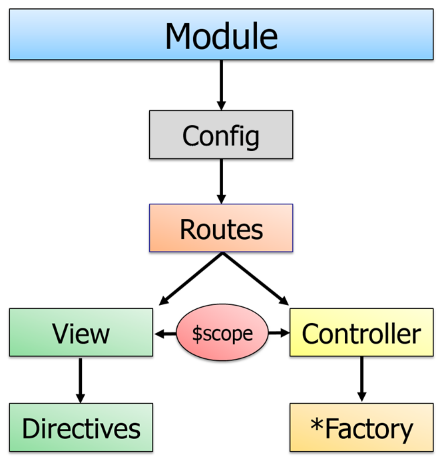
\includegraphics[width=0.5\textwidth]{arqIonic.png}
 \captionsetup{justification=centering,margin=2cm}
 \caption{Arquitectura de Ionic, adoptado para la realizac'ion del proyecto Fuente: Introducci'on a ionic\cite{Gallego}}
\label{fig:Ionic}
\end{figure}

\section{Herramientas extras}
Para el presente proyecto se ha utilizado algunas herramientas extras como ser: cordova, pouchDB, json web token y localstorage.

\subsection{Framework cordova}
Cordova es un framework de c'odigo libre para desarrollo m'ovil que nos permite usar est'andares de tecnolog'ias web como HTML5,CSS3 y Javascript. Se basa en los enlaces de API's compatibles para acceder a las capacidades del dispositivos como sensores, red, etc. En la figura \ref{fig:arqCordova} se muestra arquitectura de Cordova.

\begin{figure}[H]
\centering
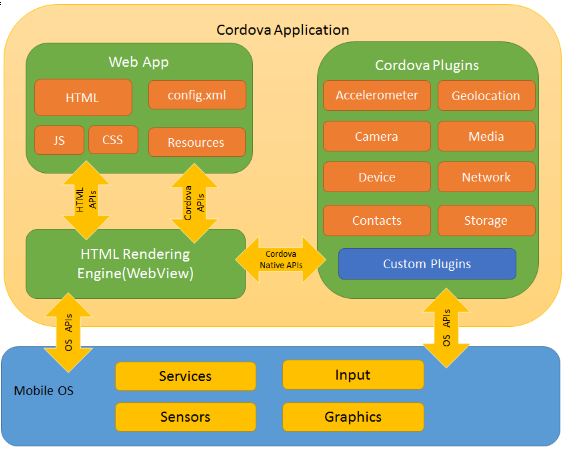
\includegraphics[width=0.3\textwidth]{arqCord.png}
\captionsetup{justification=centering,margin=2cm}
\caption{Arquitectura de cordova, adoptado para la realizac'ion del proyecto Fuente: Arquitectura de cordova\cite{Cantabriatic}}
\label{fig:arqCordova}
\end{figure}

Para el presente proyecto se utiliza cordova y se agrega su librer'ia al proyecto despu'es se instalan los plugins necesarios.

\subsection{PouchDB}
PouchDb es una capa de otras base de datos y se almacenan en el navegador esto permite guardar los datos a lado del cliente y se implementa en el lenguaje de JavaScript. La estructura de pouchdb se representa en la siguiente figura \ref{fig:pouchDB}.\cite{Pouch} 
\begin{figure}[H]
\centering
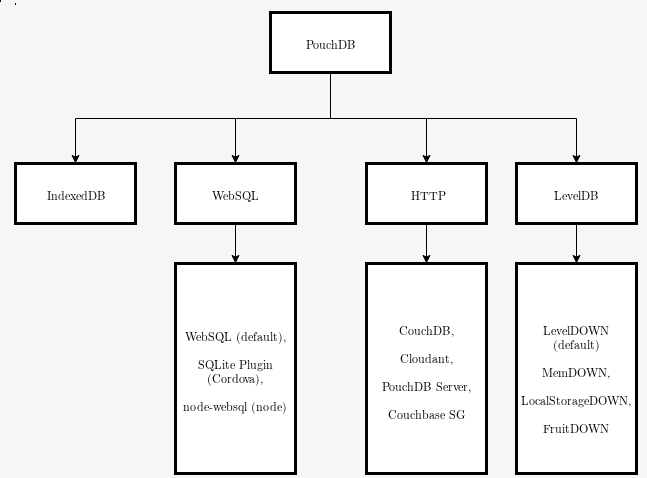
\includegraphics[width=0.3\textwidth]{pouchDB.png}
\captionsetup{justification=centering,margin=2cm}
\caption{Adaptadores de PouchDB, adoptado para la realizac'ion del proyecto Fuente: Antecedente de pouchdb\cite{Pouch}}
\label{fig:pouchDB}
\end{figure}

Seg'un la p'agina oficial de pouchDB es una base de datos NoSQL. El uso de esta API, podemos construir aplicaciones que funcionan fuera de sin conexi'on a internet y con conexi'on a internet. PouchDB utiliza WebSQL y IndexedDB internamente para almacenar los datos. 

%Para el presente proyecto se ha utilizado la capa del adaptador de websql, se explica a continuaci'on.

\subsection{Base de datos websql}
Es una herramienta para internet e intranets que facilita el acceso a base de datos relacionada con la web. Integra la tecnolog'ia  del cliente y abre la sybase el c'ual permite que los datos de la fuente se incorporen din'amicamente en la p'agina web. En la siguiente figura \ref{fig:websql} se representa la base de datos websql.
\begin{figure}[H]
\centering
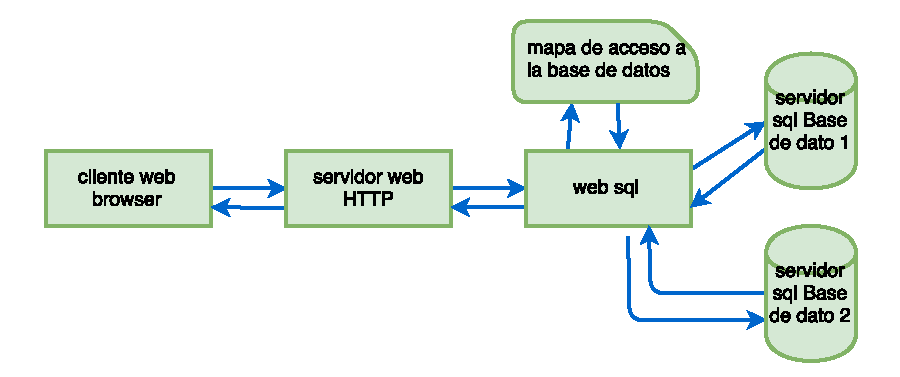
\includegraphics[width=0.6\textwidth]{websql.pdf}
\captionsetup{justification=centering,margin=2cm}
\caption{Base de datos websql, adoptado para la realizac'ion del proyecto Fuente: Adaptador de websql \cite{Websql1997}}
\label{fig:websql}
\end{figure}

\subsection{Almacenamiento local}
Es una propiedad de HTML5 web de almacenamiento, que permiten almacenar datos en nuestro navegador web denominada localstorage.
Guarda la informaci'on que permanece almacenada por tiempo indefinido, sin importar que el navegador se cierre. Tiene las siguientes caracteristicas, almacenar entre 5MB y 10MB de informaci'on, est'a almacenada en la computadora del cliente y no es enviado en cada petici'on del servidor, previene perdidas de informaci'on cuando se desconecta de la red y la informaci'on es guardada por dominio web \cite{Cardenas2015}.
\subsection{Interceptor}                                                                                                                                                                                                                                              
El interceptor utiliza el servicio de \textit{http} el c'ual permite la comunicaci'on con el servidor y captura cada petici'on y lo manipula a trav'es del \textit{httpProvider} es el que registra el contenedor del arreglos y ofrece un servicio regulador.
\subsection{Json web token}
Json web token es un m'etodo abierto y est'andar para representar las  reclamaciones de forma segura, entre dos partes que comparten informaci'on y autentificaci'on moderna, de m'ovil. El c'ual tiene una estructura representada en la figura \ref{fig:jwt}.
\begin{figure}[H]
\centering
\includegraphics[width=0.6\textwidth]{jwt.pdf}
\captionsetup{justification=centering,margin=2cm}
\caption{Json web token, adoptado para la realizac'ion del proyecto Fuente: Elaboraci'on propia}
\label{fig:jwt}
\end{figure}

Estos son las herramientas extras como se han mencionado anteriormente estas se utilizan para el presente proyecto los c'uales son compatibles con el framework ionic.